%%%%%%%%%%%%%%%%%%%%%%%%%%%%%%%%%%%%%%%%%%%%%%%%%%%%%%%%%%%%%%%%%%%%%%%%%%%%%%%%
% Related Works
% * Expand Touch Surface subsection
% - Show a picture of Wordle (A section of the thesis maybe)
% - Show a picture of WordsEye
% - Probably want to quote Carpendale's work on Elastic Framework
%%%%%%%%%%%%%%%%%%%%%%%%%%%%%%%%%%%%%%%%%%%%%%%%%%%%%%%%%%%%%%%%%%%%%%%%%%%%%%%%
\chapter{Literature Review}
There are primarily six different research areas that are relevant to our work. 
The fundamentals of information visualization, a process of transforming
data into interactive graphic, forms the basis of our work on text
summarization. Section 2.2, Descriptive rendering, reviews several
text-to-scene applications. A discussion of why NPR is beneficial is next, followed by recent examples of
visualizations that combine abstract and concrete concepts. Next, we review
the role of using lens as a focus+context interaction technique. Finally, we
review in brief the designs for touch interfaces.
  
%%%%%%%%%%%%%%%%%%%%%%%%%%%%%%%%%%%%%%%%%%%%%%%%%%%%%%%%%%%%%%%%%%%%%%%%%%%%%%%%
\section{Fundamentals}
Visualization revolves around the process of mapping and representing data or
concepts graphically such that they are visible to the human eye. Visualization, 
in theory,  takes advantage of the human perceptual system to rapidly understand
what the data is communicating to the readers. 

Foremost we want to recognize that human visual system is limited; we
can only perceive a small fraction of the entire spectrum of light, and of our
field of vision, only a small area is truly in focus. However, there is a small
set of visual properties that can be detected extremely rapidly (comparatively
to other sensory systems) and accurately by low-level perceptual system known as
preattentive processing~\cite{WAR2004b}. In theory, this perceptual system
deals with the extraction of specific graphical features without the need to 
consciously focus attention on the details, allowing viewers to spot salient and 
outlier data in a single glimpse. For example, picking out a red circle 
out of a group of blue circles is considered instantaneous, barring any visual 
abnormalities. In terms of design, exploitation of preattentive processing can 
greatly increase the rate of comprehension and ease of use.

For establishing clear visual communication, it is crucial to have a set of
visual building blocks that can be grouped and arranged to convey information. Much of
the initial work came from the field of cartography, particularly with the ideas
of marks and visual variables from Bertin~\cite{BER1983a}. Bertin defined seven
variables, including position, size, shape, value, colour, orientation and
texture. Each visual variable can have certain characteristics that can be used
to determine which of the seven visual variables is the most appropriate visual
representation. These characteristics include properties such as selective,
associative, quantitative, and ordered. A summary table below outlines the
relationship between each variable and its attributes.

\begin{table}[h]
\centering
\begin{tabular}{|l|l|l|l|l|l|l|l|}
\hline
 & Position & Size & Shape & Value & Colour & Orientation & Texture  \\  
\hline
\hline 
Selective &  Yes & Yes & Maybe & Yes & Yes & Yes & Yes \\ 
\hline
Associative &  Yes & Yes & Maybe & Yes & Yes & Yes & Yes \\
\hline
Quantitative &  Yes & Maybe & No & No & No & No & No \\
\hline 
Ordered &  Yes & Yes & No & Yes & No & No & No \\
\hline
%Length & Yes & Yes & Maybe & Yes & Yes & Yes & Yes \\
%\hline
\end{tabular}\caption{List of visual variables and
their characteristics}\label{table:VisualVariable}
\end{table}


With the building blocks in place, the next step is a formal process for
building a visualization system. There are several key
contributions in this area. More specifically, the visualization pipeline from Card \etal
~\cite{Card1999} describes a step-by-step process of data manipulation and
mapping as follows:
\begin{itemize}[noitemsep]
  \item Analysis: Normalization of raw data for visualization
  \item Filter: Select subsections of data to be visualized
  \item Mapping: Find the appropriate visual representations
  \item Rendering: Transform data into image data
\end{itemize}
For an interactive visualization, these stages are not a linear, one-off
process. The stages of Filter, Mapping and Rendering form a repetitive loop
as the users change parameters to explore different parts of the visualization.
The next part is finding interesting information within the visual presentation,
it is often through exploration that enables users to find and extract
interesting data. One process of facilitating useful graphical-based exploration
is advocated in Shneiderman's ``information seeking
mantra"~\cite{Shneiderman1996} and can be broken down into these specific tasks:
\begin{itemize}[noitemsep]
  \item Overview: See and summarize the entire collection
  \item Zoom: Zoom in on items of interest
  \item Filter: Removal of uninteresting items
  \item Detail-on-Demand: Select item/group and get details when needed
  \item Relate: View how an item relates to others
  \item History: Keep a history of actions to support undo and redo
  \item Extract: Allow extraction of subsections
\end{itemize}
Each task can then be further broken down by different types of interaction
techniques. Careful consideration should also go into each task to determine if
it is actually appropriate for the data and problem at hand.



%\textbf{Summary:} In our system, we are mostly concerned with the exploration
% of data, taking advantage of people�s ability to see colour and proximal objects. We follow 
%Shneiderman�s information seeking mantra in spirit: we have no support for 
%history or extraction functions, though these could be interesting directions 
%for our future work. 



%%%%%%%%%%%%%%%%%%%%%%%%%%%%%%%%%%%%%%%%%%%%%%%%%%%%%%%%%%%%%%%%%%%%%%%%%%%%%%%%
\section{Descriptive Rendering}
Descriptive illustration can be considered to be a sub-field of computer
graphics, which focuses on static illustrations or an animated sequence of
images based on text input. It can be considered as a text-analytic tool because
it renders the text in a literal sense or through some kind of interpretive
representation. Systems that attempt to do literal renderings are concerned
with understanding of natural languages, whereas interpreted rendering systems
tend to involve user intentions. Here we look at several examples. 

Though strictly speaking not a text-to-scene application, the IBIS application
from Seligmann and Feiner renders a \threed scene based on a set of
user-provided rules~\cite{Seligmann1991}. These rules specify which object and locations in the \threed scene have higher degrees of interest. 
The application itself evaluates these rules and determines the optimal viewing perspective, andd
the application adjusts the lighting conditions as a way to draw attention to
specific details in the scene. To our knowledge this is one of the first systems
where a preconstructed scene can be modified by text input.
 

One of the most fully-realized text-to-scene generation applications is
WordsEye~\cite{Coyne2001}. WordsEye uses a combination of grammatical rules 
and heuristics to determine subjects and their actions. These subjects are
mapped against a large repository of \threed models, and the verb actions are mapped to 
predefined poses. One of the interesting features WordsEye strives for is the
preservation of spatial relations among subjects in the text, for example: ``The cat is on
the table. The cup is on the cat.'' will render a cup on top of a cat on top
of a table (See Figure \ref{figure:wordseye}). However, WordsEye is limited by
the inherent ambiguities in written language and the accuracy of its semantic interpretation. WordsEye also works best for
a single document, and is not meant for collections of text.

    % === Figure ===  
	\begin{figure}
	 \centering  
	 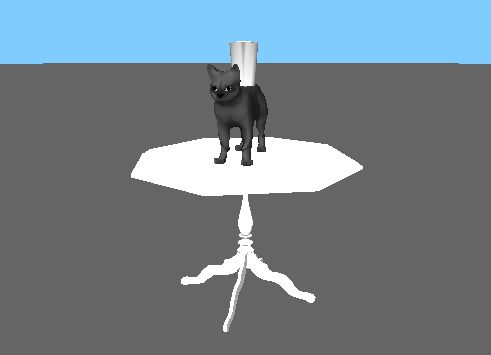
\includegraphics[width=\columnwidth]{wordseye.jpg}  
	 %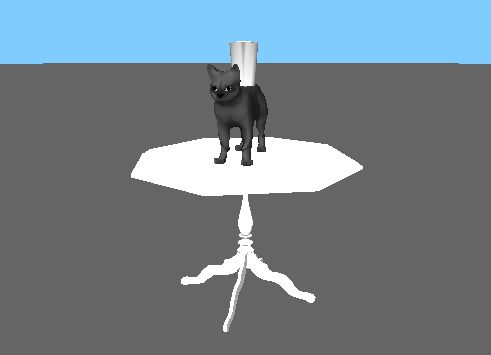
\includegraphics[scale=1.0]{wordseye.jpg}  
	 \caption[WordsEye]{WordsEye rendering of ``The cat is on the table. The cup is
	 on the cat.''}
	 \label{figure:wordseye}
	\end{figure} 
	% ==============


Another example of text-to-scene generation is CarSim~\cite{Akerberg2003},
which uses a similar logical processing and rendering process, but is
specifically designed to deal with the recreation of car accidents by parsing
traffic accident reports. Where CarSim differs is that it tries to generate an
animated sequence by inferring the speed and direction of vehicles from the text
content. However, it is less concerned with the literal representation of the car, but
rather it concentrates on the situation surrounding the incident.

    % === Figure ===  
	\begin{figure}
	 \centering  
	 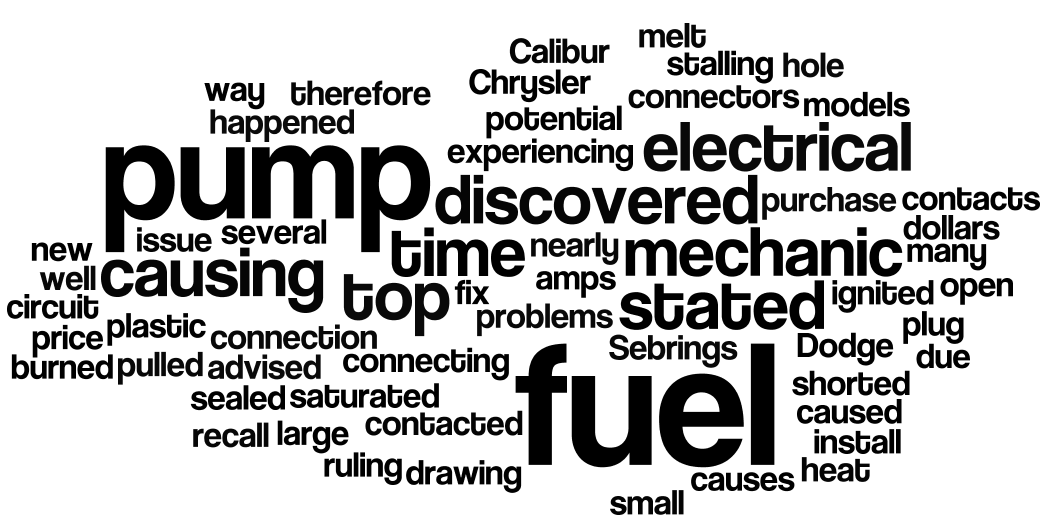
\includegraphics[width=\columnwidth]{wordle1.png}  
	 %\caption[Wordle]{A typical Wordle layout~\cite{VIE2009a}. \copyright 2009,
	 % IEEE. Reprinted with permission.}
	 \caption[Wordle]{A Wordle rendering of a vehicle complaint report.}
	 \label{figure:wordle}
	\end{figure} 
	% ==============
 
 

%So far, the discussion have been around examples where the renderings are based
%on the literal meaning of the text. On the other side are interpretive
%renderings, where the images produced are not necessarily the ground-truth of
%the text, but often produced with artistic flares and particular theme in mind.

On the interpretive side, a popular example is the web-based application called
%Wordle(http://www.wordle.net). Unlike the systems mentioned above, Wordle does
Wordle~\cite{VIE2009a} (See Figure \ref{figure:wordle}). Unlike previous systems
mentioned above, Wordle does not perform any semantic inferences on the underlying text, it rather collects frequency
statistics of each word token and encodes the frequencies as font sizes.
Unlike the closely related tag cloud, Wordle offers more creative freedom in
varying typography and colours, which are all interactively chosen by the user.
Thus it is possible to create interpretive art works based on social and
cultural norms, for example using the green colour to represent topics about
money and finance. Later variations such as Tagul took this idea further by
binding the placement of the words to specific geometric shapes and outlines,
which further strengthens how people can create their own interpretations and
expose the underlying themes~\cite{tagul}. For example, a text article about
love can be place inside a shape of a heart, instilling the idea that it is
emotionally based. However, because these creations are not usually linked to
their original text, it can be questionable whether these are proper tools for text analysis. 
 

Another example is calligraphic packing~\cite{Xu2007}, which takes a more
liberal, artistic approach. This research visualizes single words by distorting
individual glyphs to fit into \twod regions. Creative freedom is given to the
people to choose which image best represents the word, as well as the amount of
acceptable distortion. However, due to concentration on artistic style, the
legibility of the actual words after the distortion transformation is not guaranteed.


%\textbf{Summary:} Unlike WordsEye and CarSim, we start with a scene that is
%pre-constructed, that is, we know ahead of time the subjects in our text 
%documents and can place them into \threed space. While it is interesting to use 
%grammatical approach to grab context, we found it more generalizable to use a 
%dictionary approach similar to Wordle for parsing text because we iterate 
%over thousands of documents.


%%%%%%%%%%%%%%%%%%%%%%%%%%%%%%%%%%%%%%%%%%%%%%%%%%%%%%%%%%%%%%%%%%%%%%%%%%%%%%%% 
\section{Non-Photorealistic Rendering}
Since the infancy of computer graphics, researchers have long been looking at
ways to render photorealistic images that are nearly
indistinguishable from a photograph taken by a camera. In recent years,
however, another area of computer graphics research has been looking in the
opposite direction: Non-Photorealistic Rendering. Non-Photorealistic Rendering can be 
described as any computer generated graphics that do not involve the accurate 
simulation of the behaviour of light. While photorealism has long been the holy
grail in graphics research, there are compelling reasons for using NPR
techniques. First, NPR images are judged based on their ability to
communicate a specific message to their viewers, thus they are driven to
emphasize features in a scene or some underlying attributes~\cite{Gooch2001}.
This is in contrast with photorealistic rendering where the goal is to compare
the rendering against a ground-truth image. Second, often times it is
undesirable to preserve a high degree of realism, reflections, shadows
and other natural lighting phenomena may obstruct or create
false-positive surface details. NPR can choose to ignore the natural laws of physics, and instead
choose to focus on different abstractions such that the illustration can be
meaningful to people from different fields. Since there are multitudes of
possibilities in NPR, this section solely focuses on prior works that related
to our work here, or served as our inspirations.

%\daniel{Perhaps repace toonshading with half-toning? more relevant because it
%mentiones textures} 

Images found in technically written materials, or that of
instructional manuals are quite different than those found in photo scrapbooks. The key point, as
stated above, is that communication is valued above realism. Early works by
Gooch \etal~uncovered common themes in technical illustrations and ways to
automate some of these properties~\cite{Gooch1998}. Gooch \etal~modified the
conventional shading algorithm to use a two-tone approach that shifts from
warm-colours to cool-colours, in addition, they added edge lines and removed
shadows. Illustrations created in this fashion have major benefits over
photography. One, strong lighting effects under conventional shading model are
reduced, thus preserving the surface details under the light patches. Two, the
removal of shadow regions shows the hidden details that were not previous
visible. Other NPR shading techniques also exist, for example 
those that emulate the simplistic cartoon styles known as
cel-shading and toon-shading~\cite{Lake2000}. Generally speaking, cel-shading
and toon-shading map the intensity of light from a continuous function into discrete
values, creating distinct contours where the values change as if shaded by a
marker. Still other works look at the simulation of physical materials,
for example textures as halftones to simulate stylistic artistic
sketches~\cite{Freudenberg2002}, and pen-and-ink
illustrations~\cite{Salisbury1994}. However it is semi-automatic as some human
input is required for the right combination of textures, normal maps and other
special effects.
   

Another major benefit of NPR is that it can be used to simplify or
accentuate geometric features. By taking advantage of visual perception
capabilities of seeing continuities and surfaces as dictated by Gestalt Principals~\cite{WAR2004b}, humans can see and complete entire shapes with just a few
geometric primitives. Feature extraction, which revolves around the detection
and isolation of shapes and primitives, can be used to achieve this goal. 

%Feature extraction is one way to achieve this goal by
%simplifying an image down to geometric primitives of lines and curves.

Feature extraction can be done in either \twod or \threed spaces. The \twod
algorithm is image based, and based upon calculating the a discontinuity value
of a pixel against its neighbouring pixels~\cite{Gonzalez2002}. The
discontinuity can take on several types, for example colour, normal and depth. A
square matrix, called a kernel, is used as a convolution operator to evaluate a
measure of discontinuity of each pixel in the image. Any pixels with a
discontinuity measure that fall below a specified threshold are discarded, the
remaining pixels are collected and aggregated into higher level geometric
primitives. In \threed space, features can be classified under the broad
categories of ridges, valleys and  silhouettes.
Ridges are formed by two front facing polygons with dihedral angle between 0 to
180, similarly, valleys are front facing polygons with dihedral angle between
180 to 360, both of these are exclusive, as an angle of 0 or 180 results in a
flat surface. Lastly, silhouette edges are formed by the shared edge of
front-facing polygons and back-facing polygons. Raskar~\cite{Raskar2001}
computes these \threed features without connectivity information by extruding
additional faces per polygon. In addition, since the features are geometric
quads, additional processing can be performed on these quads such that they can
be rendered in a multitude of ways. However, because the extrusions are
performed on all sides of the polygon, the algorithm introduces extraneous
faces, which are hidden by existing geometries through back-face culling.
Hermosilla~\cite{Hermosilla2009} took this idea further by moving the extrusion
process to modern graphic pipeline's geometry shader, removing the need to perform 
the computations on the CPU. It should be noted that in an interactive environment,
geometric features are generally view dependent in both \threed and \twod
scenarios, and this usually means that feature extraction operations need to 
run on a per frame basis.
 

When it comes to expressiveness, NPR rendering styles can be used to convey a
variety of semantics. Of particular interest to us is the idea of uncertainty:
graphics that are visible to the viewer, but also convey a sense of error
and inaccuracy. Research in ancient architectural
reconstructions found that straight, solid
strokes convey a higher degree of certainty than strokes that are drawn faded and
curved~\cite{Masuch1998, Strothotte1999}. The relevance here to our work is
that we use this type of technique to convey objects that are not in the focused
context.


    % === Figure === 
	\begin{figure}
	 \centering  
	 %\includegraphics[width=\columnwidth]{copyright/viola.png}  
	 \includegraphics[scale=1.0]{copyright/viola.png}  
	 \caption[Importance-Driven Volume Rendering]{Importance-Driven Volume
	 Rendering~\cite{Viola2004}.
	 \copyright 2004, IEEE. Reprinted with permission.}
	 \label{figure:viola}
	\end{figure} 
	% ==============

%One prominent research came from an
%importance-driven function that can be used to determine the visibility of
%objects~\cite{Viola2004} (See Figure \ref{figure:viola}). 

Another branch of non-photorealistic rendering deals with semantic segmentation
of objects in the scene. For example illustrations found in science and
medical literature where specific parts are accentuated using different colours.
This is done in order to differentiate focus and non-focus regions in the final
illustration. These types of NPR techniques are particularly prominent in the 
Scientific Visualization community, where they deal with visibility issues to
ensure that semantically important objects are easily visible and to provide
features to deal with occlusion. For example, Viola \etal~used an
importance-driven function to determine the visibility of
objects~\cite{Viola2004}. In their work numerical scores
are assigned to volumetric components such that more important objects are
rendered more opaque than objects of lesser importance (See Figure
\ref{figure:viola}). A screen door transparency technique is introduced to
ensure overall visibility by rendering holes into the outermost volumetric
layers. The idea of segmentation and context is taken further by Tietjen \etal,
who describe a segmentation scheme that partitions different volumes into
focus, near focus and context categories~\cite{Tietjen2005}, with the following semantics:
\begin{itemize}[noitemsep]
  \item Focus object: Current focus and is emphasized.
  \item Near focus object: Object for understanding spatial location or
  interrelations.
  \item Context Object: All other objects in the scene.
\end{itemize}
The segmentation allows for further accentuation of specific regions, while
still providing enough background context to understand the subject matter.

%In action, focus, near-focus and context objects can be interactively changed
%and take on different artistic styles.



%%%%%%%%%%%%%%%%%%%%%%%%%%%%%%%%%%%%%%%%%%%%%%%%%%%%%%%%%%%%%%%%%%%%%%%%%%%%%%%% 
\section{Integrated Visualization}
Traditionally, Information Visualization deals with abstract data, while
Scientific Visualization deals with visualization of
concrete subjects such as physical or anatomical objects. However, while these
are two distinct communities, the division is not always obvious. Many
applications combine elements and techniques from both fields, though the two
sides remain separate disciplines. As data becomes more heterogeneous, new
approaches for data visualization make the case of whether the boundary should
exist or not, as illustrated by recent attention to discuss the similarities and
differences between the two groups~\cite{Hauser2005, Weiskopf2004}. The SciVis
community in particular has adopted techniques and practices that are
traditionally in the InfoVis community. A well-known example is the volumetric
visualization from Doleisch \etal, which uses multiple coordinated views in addition to 
linking and brushing techniques to further help the exploration
process~\cite{Doleisch2003}.

    % === Figure === 
	\begin{figure}
	 \centering  
	 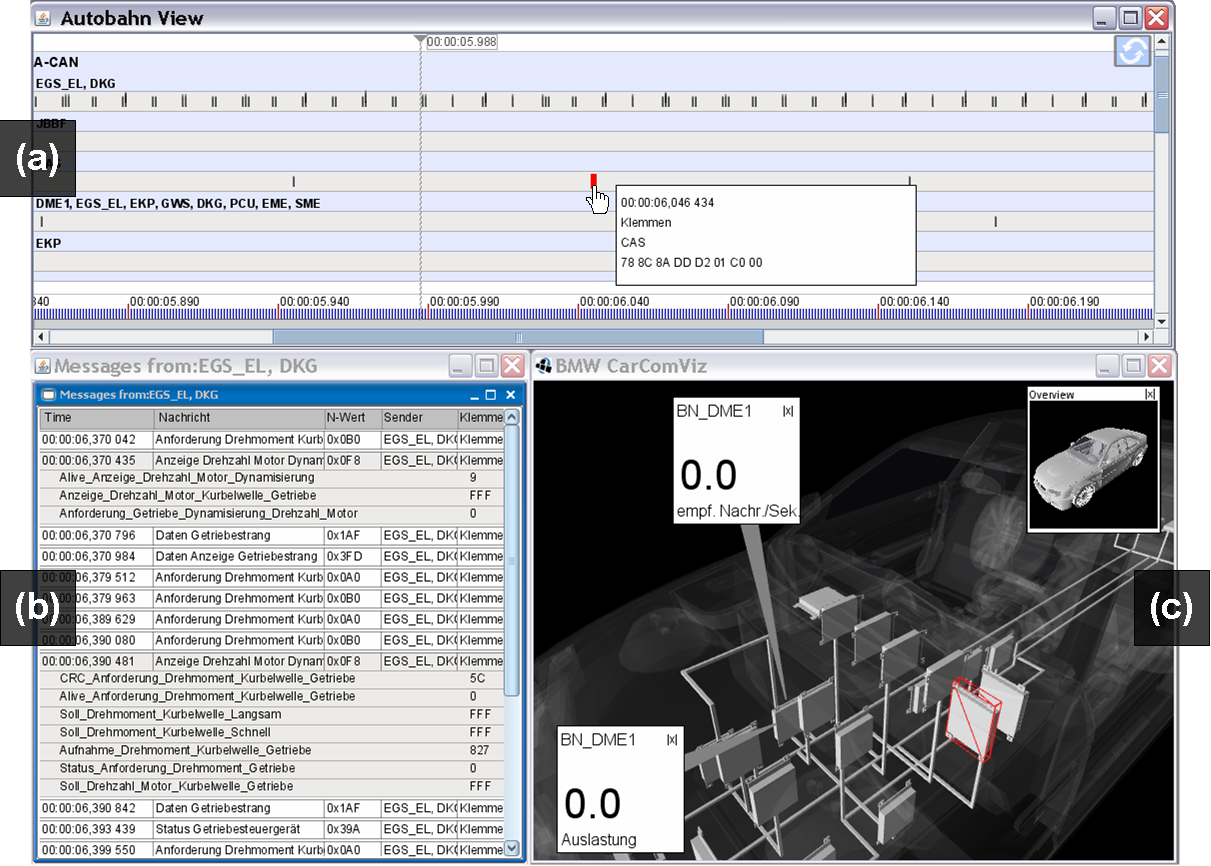
\includegraphics[width=\columnwidth]{copyright/sedlmair.png}  
	 \caption[CarComVis]{User interface for CarComVis~\cite{Sedlmair2009}.
	 \copyright 2009, Springer. Reprinted with permission.}
	 \label{figure:sedlmair}
	\end{figure} 
	% ==============

For a more hybrid space approach between InfoVis and SciVis,  Balabanian \etal~
placed hierarchical renderings of human anatomy inside an interactive
balloon-tree graph~\cite{Balabanian2010}. In this graph, each anatomical object
occupies a node, and is arranged by logical hierarchy. The colours, size and arrangement of the nodes are dictated by abstract 
semantics, such as what is currently selected, filtering operations, 
and relations among the anatomical parts. The \threed rendering supports SciVis
operations such as viewing, slicing and picking of objects. Changes are linked
and propagated across relevant nodes and volume renderings.


In the InfoVis space, research by Sedlmair \etal~examined enriching
InfoVis visualizations with \threed models~\cite{Sedlmair2009}.
In this work, they presented two applications, CarComVis, which allows users to
explore intercommunication among vehicle components, and LibVis, which explores
environmental reading in a library setting. Neither one is explicitly about
physical objects, but contains inherent spatial information for reconstructing a
\threed representation: An automobile model for CarComVis and a virtual library
environment for LibVis. Sedlmair \etal~explore different types of integration
techniques, including the usage of multiple coordinated views and a total immersion 
environment where the user is in a virtual world. Subjective feedback 
from their study suggested a strong desire for integration of \threed
visualizations into traditional visualization and work flow. Our work in this
thesis is perhaps mostly closely associated with CarComVis (see Figure
\ref{figure:sedlmair}), however our renderings are driven by unstructured text,
and our interactions are directly applicable to the visualization itself rather
than through multiple coordinated views.

%\textbf{Summary:} We take an approach similar to CarComVis [Seldmair2009], we
%generated a virtual vehicle based on the components mentioned in our dataset. However, rather 
%than using a coordinated views for information seeking, our interactions are more 
%tightly coupled with the \threed visualization. Also, our visualization style is
%based on the context of the dataset, rather than using a fixed visualization.

%%%%%%%%%%%%%%%%%%%%%%%%%%%%%%%%%%%%%%%%%%%%%%%%%%%%%%%%%%%%%%%%%%%%%%%%%%%%%%%% 
\section{Focus+Context Techniques}
Focus+Context is a well-known and practiced technique in InfoVis; it is used to
draw attention to particular areas of interest while maintaining a certain degree of contextual 
information. There are various ways to discriminate these areas. For example 
Hauser reviewed the general approaches and demonstrated the usage of colour,
spatial-location, opacity, and other resource~\cite{Hauser2006}.
One interesting use of the focus+context technique is the idea of using lenses; the
lens traces back to a real world metaphor of a magnification lens, where the
area directly under the lens are distorted and enlarged by the optics. In
interactive visualization, the lens acts as a specialised user interface widget,
where the data graphics under the lens undergo a graphical transformation in
order to represent different semantics.


Fisheye Lens is a technique for enlarging
details on a \twod image, for example on digital maps and circuit
diagrams~\cite{Sarkar1992}. Much like its real world counterpart, a fisheye lens technique creates an ultra-wide viewing perspective that
creates a distortion displacement under the lens. The amount of displacement 
is controlled via a drop-off function that determines the degree of enlargement 
and shrinkage, typically with the central part of the lens enlarged while area
regions near the circumferences shrink to compensate. There are a
few usability issues with a fisheye lens, and likely the same issue applies to all
lenses that undergo geometric distortion: distorted graphics are more
difficult to read, and it is harder to tell where the focus is, because the
lens itself may occlude nearby objects which the viewer use as navigational cues.

Although not directly a focus+context scenario, the original publication of
using a flexible and multipurpose virtual lenses likely came from Bier \etal's Magic
Lenses~\cite{Bier1993}. The lens is composed of various widgets arranged on a
semi-transparent overlay, where the interaction with a widget affects the
immediate graphical region beneath it, for example changing the colour or size
of the graphical region.


%Although not directly a focus+context scenario, the original idea of using a
%flexible and multipurpose virtual lens likely came from research by Bier \etal,
%where a transparent overlay can be used to modify the appearance and behaviour
%of objects underneath the overlay panel~\cite{Bier1993}. Perhaps more
%significantly, the lens acts as an interactive layer, where actions can be send
%through the lens directly to the objects beneath it.


NPRLens follows up on the MagicLens metaphor from Bier
\etal, allowing users to interactively create images in a non-photorealistic
style~\cite{Neumann2007a}. NPRLens performs image processing on the \twod
projections of objects in \threed space. Graphical data points are first projected to screen space,
collected and aggregated into higher level graphical constructs such as line
segment and curve primitives. These can then be further manipulated such as
stretching, shrinking or changing the stroke styles of each primitive unit.


\threed MagicLens~\cite{Viega1996} is likely the first foray of the lens idea
taken into three dimensional space, and unlike the previously mentioned works,
MagicLens works with viewing volumes rather than \twod image maps. The lens in this scenario slices
the scene into different frustum volumes, each volume is then rendered separately 
and then recomposed together to create the final scene. This technique allows 
people to create interesting effects, for example exposing the skeletal 
structures of multi-layered objects. With more advanced hardware features, it is
possible to buffer the rendering into textures and combine them at a later
stage, rather than physically cutting the scene in volumes, this is the
technique that we use in our work.


Other than stylization and distortion techniques, the same lens metaphor can
also be used as a way to augment information seeking. In this context the lens 
is an exploration device that exposes hidden data points, or data points that 
cannot be feasibly displayed in a readable manner. Generally these cases arise
because of overlapping points, or when there are too many points on the screen,
making labelling of all points impractical as they introduce too much visual
clutter. Excentric Labeling~\cite{Fekete1999} uses the lens metaphor to deal
with densely populated data points on a \twod illustration. Data points are not
labelled, instead, when the lens is hovered over the locations that contain data
points, line segments are extended from the data points outward towards the
circumference of the lens. The actual text labels and descriptions are drawn
along the circumference, allowing viewers to make the connection between
graphics and text. The lens itself is movable which allows for exploration of
interesting regions. Extended Excentric Labeling~\cite{Bertini2009} (Figure
\ref{figure:bertini}) further extends on the idea by creating additional
interactions with the lens, dynamic overviews are shown inside the lens as
miniature graphs summarizing of objects under the lens. The labels are
scrollable to allow exploration of dense areas without overcrowding screen
space, the layout of labels and the extending lines are also altered to minimize
crossings which can cause additional visual complexity.
 
    % === Figure === 
	\begin{figure}
	 \centering    
	 %\includegraphics[width=\columnwidth]{copyright/bertini.png}  
	 \includegraphics[scale=1.0]{copyright/bertini.png}  
	 \caption[Extended Excentric Labelling]{Extended Excentric
	 Labelling~\cite{Bertini2009}.
	 \copyright 2009, The Eurographics Association and Blackwell Publishing.
	 Reprinted with permission.}
	 \label{figure:bertini}
	\end{figure} 
	% ==============


%While both Excentric and Extended Excentric Lens operate in \twod space, there
%are some researches with that takes the same ideas into environments that are
%composed of \threed objects. 

While the techniques described above are largely applied to \twod applications, there are
applicable \threed focus+context techniques. Sonnet \etal~created a medical volume rendering system where the lens takes the form of a
\threed cursor~\cite{Sonnet2004}, although viewers cannot see into the cursor
itself, the cursor creates a spherical volume that pushes other volumetric objects away from the center, thus
creating more space for labels and annotations, and reduces the occlusion issues
that come naturally with \threed environment. Another system is BrainGazer, a volumetric visualization application that allows
users to draw a query path onto a segmented volume data~\cite{Bruckner2009}. The
path exhibits lens like behaviour, that is, the systems queries the objects that are in
proximity to the path drawn. Additional information about these objects is then
shown in a separate user interface panel. Our system uses a similar approach, in
that the scene we render is pre-segmented into regions of different
semantics, though we use an actual lens as the querying tool, and we deal with
geometric rather than volumetric data.

 
%\textbf{Summary:} Our approach to focus+context resembles a combination of
%approaches taken by BrainGazer, NPRLens and Excentric Labels. Like BrainGazer, we allow 
%people to form visual queries via indexing spatial location with different semantics, 
%though we take a proactive approach to highlight and link the text data back to 
%the visualization by combining ideas from NPRLens and Excentric Labels.


%%%%%%%%%%%%%%%%%%%%%%%%%%%%%%%%%%%%%%%%%%%%%%%%%%%%%%%%%%%%%%%%%%%%%%%%%%%%%%%%
\section{Design for Touch Interface}
As the cost of touch surface computing becomes cheaper, we are gradually seeing 
interactive surfaces introduced into public areas, office work environments and 
personal spaces. Interactive interfaces bring new possibilities of exchanging 
information in a walk-by scenario~\cite{Vogel2004}, allowing people to
interact with data without the need of peripheral hardware devices such as the
mouse or keyboard. Instead, people utilize their hands and fingers as
interactive mediums.

Though much of the work today deals with either collaborative or
distributed environments, the focus in this work deals with designing
surface-based gestures for a large display space. Gesture design
and classification have been looked at via crowd sourcing approaches,
leveraging public opinions to come to a consensus as to which action should be
associated with what gestures. For example, Wobbrock \etal~conducted
experiments where the consequences are given, and participants had to come up with their own appropriate gestures to cause the said
actions~\cite{Wobbrock2009}. Others, such as Hinrichs and Carpendale, looked at
how environmental and social context affect how people perform gestures
~\cite{Hinrichs2011}. In both cases, experimental results converge and they were
able to create high-level classifications. On the other hand, these
classifications are derived from independent, low-level tasks, where our
prototype looks at a specific problem from end-to-end. As such, these
classifications serve as inspirations rather than dictating our gesture
design.

Aside from classification, there are many other nuances and device specific
attributes in gesture design that one needs to pay attention to make them
more user friendly. Providing appropriate visual feedback, dealing with
false-positive/false-negative touches, and target acquisition are some of
important details for natural interactions. Much of the intricacies are outline
by Wigdor and Wixon, where they discussed design principles and other
guidelines~\cite{Wigdor2011}.


 

